\documentclass{ximera}  


%\usepackage{todonotes}
%\usepackage{mathtools} %% Required for wide table Curl and Greens
%\usepackage{cuted} %% Required for wide table Curl and Greens
\newcommand{\todo}{}

\usepackage{esint} % for \oiint
\ifxake%%https://math.meta.stackexchange.com/questions/9973/how-do-you-render-a-closed-surface-double-integral
\renewcommand{\oiint}{{\large\bigcirc}\kern-1.56em\iint}
\fi


\graphicspath{
  {./}
  {jpg}
  {ximeraTutorial/}
  {basicPhilosophy/}
  {functionsOfSeveralVariables/}
  {normalVectors/}
  {lagrangeMultipliers/}
  {vectorFields/}
  {greensTheorem/}
  {shapeOfThingsToCome/}
  {dotProducts/}
  {partialDerivativesAndTheGradientVector/}
  {../productAndQuotientRules/exercises/}
  {../motionAndPathsInSpace/exercises/}
  {../normalVectors/exercisesParametricPlots/}
  {../continuityOfFunctionsOfSeveralVariables/exercises/}
  {../partialDerivativesAndTheGradientVector/exercises/}
  {../directionalDerivativeAndChainRule/exercises/}
  {../commonCoordinates/exercisesCylindricalCoordinates/}
  {../commonCoordinates/exercisesSphericalCoordinates/}
  {../greensTheorem/exercisesCurlAndLineIntegrals/}
  {../greensTheorem/exercisesDivergenceAndLineIntegrals/}
  {../shapeOfThingsToCome/exercisesDivergenceTheorem/}
  {../greensTheorem/}
  {../shapeOfThingsToCome/}
  {../separableDifferentialEquations/exercises/}
  {vectorFields/}
}

\newcommand{\mooculus}{\textsf{\textbf{MOOC}\textnormal{\textsf{ULUS}}}}

\usepackage{tkz-euclide}\usepackage{tikz}
\usepackage{tikz-cd}
\usetikzlibrary{arrows}
\tikzset{>=stealth,commutative diagrams/.cd,
  arrow style=tikz,diagrams={>=stealth}} %% cool arrow head
\tikzset{shorten <>/.style={ shorten >=#1, shorten <=#1 } } %% allows shorter vectors

\usetikzlibrary{backgrounds} %% for boxes around graphs
\usetikzlibrary{shapes,positioning}  %% Clouds and stars
\usetikzlibrary{matrix} %% for matrix
\usepgfplotslibrary{polar} %% for polar plots
\usepgfplotslibrary{fillbetween} %% to shade area between curves in TikZ
\usetkzobj{all}
\usepackage[makeroom]{cancel} %% for strike outs
%\usepackage{mathtools} %% for pretty underbrace % Breaks Ximera
%\usepackage{multicol}
\usepackage{pgffor} %% required for integral for loops



%% http://tex.stackexchange.com/questions/66490/drawing-a-tikz-arc-specifying-the-center
%% Draws beach ball
\tikzset{pics/carc/.style args={#1:#2:#3}{code={\draw[pic actions] (#1:#3) arc(#1:#2:#3);}}}



\usepackage{array}
\setlength{\extrarowheight}{+.1cm}
\newdimen\digitwidth
\settowidth\digitwidth{9}
\def\divrule#1#2{
\noalign{\moveright#1\digitwidth
\vbox{\hrule width#2\digitwidth}}}





\newcommand{\RR}{\mathbb R}
\newcommand{\R}{\mathbb R}
\newcommand{\N}{\mathbb N}
\newcommand{\Z}{\mathbb Z}

\newcommand{\sagemath}{\textsf{SageMath}}


%\renewcommand{\d}{\,d\!}
\renewcommand{\d}{\mathop{}\!d}
\newcommand{\dd}[2][]{\frac{\d #1}{\d #2}}
\newcommand{\pp}[2][]{\frac{\partial #1}{\partial #2}}
\renewcommand{\l}{\ell}
\newcommand{\ddx}{\frac{d}{\d x}}

\newcommand{\zeroOverZero}{\ensuremath{\boldsymbol{\tfrac{0}{0}}}}
\newcommand{\inftyOverInfty}{\ensuremath{\boldsymbol{\tfrac{\infty}{\infty}}}}
\newcommand{\zeroOverInfty}{\ensuremath{\boldsymbol{\tfrac{0}{\infty}}}}
\newcommand{\zeroTimesInfty}{\ensuremath{\small\boldsymbol{0\cdot \infty}}}
\newcommand{\inftyMinusInfty}{\ensuremath{\small\boldsymbol{\infty - \infty}}}
\newcommand{\oneToInfty}{\ensuremath{\boldsymbol{1^\infty}}}
\newcommand{\zeroToZero}{\ensuremath{\boldsymbol{0^0}}}
\newcommand{\inftyToZero}{\ensuremath{\boldsymbol{\infty^0}}}



\newcommand{\numOverZero}{\ensuremath{\boldsymbol{\tfrac{\#}{0}}}}
\newcommand{\dfn}{\textbf}
%\newcommand{\unit}{\,\mathrm}
\newcommand{\unit}{\mathop{}\!\mathrm}
\newcommand{\eval}[1]{\bigg[ #1 \bigg]}
\newcommand{\seq}[1]{\left( #1 \right)}
\renewcommand{\epsilon}{\varepsilon}
\renewcommand{\phi}{\varphi}


\renewcommand{\iff}{\Leftrightarrow}

\DeclareMathOperator{\arccot}{arccot}
\DeclareMathOperator{\arcsec}{arcsec}
\DeclareMathOperator{\arccsc}{arccsc}
\DeclareMathOperator{\si}{Si}
\DeclareMathOperator{\scal}{scal}
\DeclareMathOperator{\sign}{sign}


%% \newcommand{\tightoverset}[2]{% for arrow vec
%%   \mathop{#2}\limits^{\vbox to -.5ex{\kern-0.75ex\hbox{$#1$}\vss}}}
\newcommand{\arrowvec}[1]{{\overset{\rightharpoonup}{#1}}}
%\renewcommand{\vec}[1]{\arrowvec{\mathbf{#1}}}
\renewcommand{\vec}[1]{{\overset{\boldsymbol{\rightharpoonup}}{\mathbf{#1}}}\hspace{0in}}

\newcommand{\point}[1]{\left(#1\right)} %this allows \vector{ to be changed to \vector{ with a quick find and replace
\newcommand{\pt}[1]{\mathbf{#1}} %this allows \vec{ to be changed to \vec{ with a quick find and replace
\newcommand{\Lim}[2]{\lim_{\point{#1} \to \point{#2}}} %Bart, I changed this to point since I want to use it.  It runs through both of the exercise and exerciseE files in limits section, which is why it was in each document to start with.

\DeclareMathOperator{\proj}{\mathbf{proj}}
\newcommand{\veci}{{\boldsymbol{\hat{\imath}}}}
\newcommand{\vecj}{{\boldsymbol{\hat{\jmath}}}}
\newcommand{\veck}{{\boldsymbol{\hat{k}}}}
\newcommand{\vecl}{\vec{\boldsymbol{\l}}}
\newcommand{\uvec}[1]{\mathbf{\hat{#1}}}
\newcommand{\utan}{\mathbf{\hat{t}}}
\newcommand{\unormal}{\mathbf{\hat{n}}}
\newcommand{\ubinormal}{\mathbf{\hat{b}}}

\newcommand{\dotp}{\bullet}
\newcommand{\cross}{\boldsymbol\times}
\newcommand{\grad}{\boldsymbol\nabla}
\newcommand{\divergence}{\grad\dotp}
\newcommand{\curl}{\grad\cross}
%\DeclareMathOperator{\divergence}{divergence}
%\DeclareMathOperator{\curl}[1]{\grad\cross #1}
\newcommand{\lto}{\mathop{\longrightarrow\,}\limits}

\renewcommand{\bar}{\overline}

\colorlet{textColor}{black}
\colorlet{background}{white}
\colorlet{penColor}{blue!50!black} % Color of a curve in a plot
\colorlet{penColor2}{red!50!black}% Color of a curve in a plot
\colorlet{penColor3}{red!50!blue} % Color of a curve in a plot
\colorlet{penColor4}{green!50!black} % Color of a curve in a plot
\colorlet{penColor5}{orange!80!black} % Color of a curve in a plot
\colorlet{penColor6}{yellow!70!black} % Color of a curve in a plot
\colorlet{fill1}{penColor!20} % Color of fill in a plot
\colorlet{fill2}{penColor2!20} % Color of fill in a plot
\colorlet{fillp}{fill1} % Color of positive area
\colorlet{filln}{penColor2!20} % Color of negative area
\colorlet{fill3}{penColor3!20} % Fill
\colorlet{fill4}{penColor4!20} % Fill
\colorlet{fill5}{penColor5!20} % Fill
\colorlet{gridColor}{gray!50} % Color of grid in a plot

\newcommand{\surfaceColor}{violet}
\newcommand{\surfaceColorTwo}{redyellow}
\newcommand{\sliceColor}{greenyellow}




\pgfmathdeclarefunction{gauss}{2}{% gives gaussian
  \pgfmathparse{1/(#2*sqrt(2*pi))*exp(-((x-#1)^2)/(2*#2^2))}%
}


%%%%%%%%%%%%%
%% Vectors
%%%%%%%%%%%%%

%% Simple horiz vectors
\renewcommand{\vector}[1]{\left\langle #1\right\rangle}


%% %% Complex Horiz Vectors with angle brackets
%% \makeatletter
%% \renewcommand{\vector}[2][ , ]{\left\langle%
%%   \def\nextitem{\def\nextitem{#1}}%
%%   \@for \el:=#2\do{\nextitem\el}\right\rangle%
%% }
%% \makeatother

%% %% Vertical Vectors
%% \def\vector#1{\begin{bmatrix}\vecListA#1,,\end{bmatrix}}
%% \def\vecListA#1,{\if,#1,\else #1\cr \expandafter \vecListA \fi}

%%%%%%%%%%%%%
%% End of vectors
%%%%%%%%%%%%%

%\newcommand{\fullwidth}{}
%\newcommand{\normalwidth}{}



%% makes a snazzy t-chart for evaluating functions
%\newenvironment{tchart}{\rowcolors{2}{}{background!90!textColor}\array}{\endarray}

%%This is to help with formatting on future title pages.
\newenvironment{sectionOutcomes}{}{}



%% Flowchart stuff
%\tikzstyle{startstop} = [rectangle, rounded corners, minimum width=3cm, minimum height=1cm,text centered, draw=black]
%\tikzstyle{question} = [rectangle, minimum width=3cm, minimum height=1cm, text centered, draw=black]
%\tikzstyle{decision} = [trapezium, trapezium left angle=70, trapezium right angle=110, minimum width=3cm, minimum height=1cm, text centered, draw=black]
%\tikzstyle{question} = [rectangle, rounded corners, minimum width=3cm, minimum height=1cm,text centered, draw=black]
%\tikzstyle{process} = [rectangle, minimum width=3cm, minimum height=1cm, text centered, draw=black]
%\tikzstyle{decision} = [trapezium, trapezium left angle=70, trapezium right angle=110, minimum width=3cm, minimum height=1cm, text centered, draw=black]




 
\title{Inductance} 
\author{Milica Markovic} 
\outcome{Define and calculate inductance for specific conductor configurations.}
\begin{document}  
\begin{abstract}  

\end{abstract}  
\maketitle    


\section{Magnetic flux, review of electric flux}

A conceptual definition of magnetic flux is the number of magnetic field lines penetrating a surface. 

\begin{eqnarray}
\Phi_B= N_B 
\end{eqnarray}

Mathematically, magnetic flux is defined through magnetic flux density vector B as

\begin{eqnarray}
\Phi_B= \int_S \vec{B} \cdot \vec{dS}
\end{eqnarray}

If the angle between the surface dS and B vector is the same, and the B vector is constant on the surface, we have that $\Phi_B=B S$, or $B=\frac{\Phi_B}{S}$. Vector $\vec{B}$ is called magnetic flux density, just like in electrostatics, vector $D=\frac{\Phi_E}{S}$ was called electric flux density vector.

Magnetic flux density vector $\vec{B}$ and magnetic field vector $\vec{H}$ are related through the magnetic permeability of the material $\mu$.

\begin{eqnarray}
\vec{B} = \mu \vec{H}
\end{eqnarray}

Similarly, in electrostatics, the electric flux density vector $\vec{D}$, and electric field vector $\vec{E}$ are related through the electric permittivity of the material $\epsilon$.

\begin{eqnarray}
\vec{D} = \epsilon \vec{E}
\end{eqnarray}

\section{Definition of inductance}
 
 A simplified, conceptual definition of inductance is the number of magnetic field lines around a conductor, divided by the current in a wire.
 
 \begin{eqnarray}
 L=\frac{N_B}{I}
 \end{eqnarray}
 
 For example, if we have five magnetic field lines around the wire that carries the current 1A, then the inductance is L=5/1=5\,H. If we have another wire that makes ten magnetic field lines around it for the same current flowing through it of 1A, then the inductance of this wire is L=10\,H. This type of inductance is called self-inductance. We will talk about mutual inductance in the section below.

The scientific definition of inductance is the ratio of magnetic flux to the current that produced it.

\begin{eqnarray}
L=\frac{\Phi}{I} \\
L=\frac{\int_S \vec{B} \cdot \vec{dS}}{I}
\end{eqnarray}

\section{Magnetostatic energy}

Inductors store magnetic energy. Capacitors store electric energy. The magnetic energy stored in an inductor is

\begin{equation}
W_m=\frac{1}{2} L I^2
\end{equation}

The total magnetic energy stored in a volume is

\begin{equation}
W_m=\frac{1}{2}\int_v \vec{B} \cdot \vec{H} \, dv 
\end{equation}

B is the magnetic flux density, H is the magnetic field, and v is the volume in which the energy is stored. 

By equating the above two equations, we can find the inductance of an inductor as

\begin{equation}
L=\frac{1}{I^2} \int_v \vec{B} \cdot \vec{H} \,dv 
\end{equation}

In linear, homegenous materials $\vec{B} = \mu \vec{H}$, the equation simplifies to

\begin{equation}
L=\frac{\mu}{I^2} \int_v H^2 dv 
\end{equation}

In the electrostatics section, we found that the capacitance is found as


\begin{equation}
C=\frac{\epsilon}{V^2} \int_v E^2 dv 
\end{equation}

V is the potential difference, v is the volume where electric energy is stored, and E is the electric field.

\begin{example}
\section{Deriving inductance for a coaxial cable}

Derive the inductance of a length h of a coaxial cable carrying current I. The inner radius of the coaxial cable is a, and the outer radius is b. 

\begin{solution}
In the previous section, we derived the magnetic field around an infinite straight line carrying current $H(r)=\frac{I}{2 \pi r}$. The magnetic field between a coaxial cable's inner and outer conductor is the same as an infinite straight line's magnetic field.

Using the equation for the magnetic field and integrating throughout a section of the volume between the inner and outer conductor of the coaxial cable, we get


\begin{equation}
L=\frac{\mu}{I^2} \int_v \frac{I}{2 \pi r}^2 dv 
\end{equation}

since the only variable is the distance r, and the unit volume in cylindrical coordinates is $dv=r dr d\theta dz$, the integral simplifies to


\begin{equation}
L=\frac{\mu}{I^2} \int_0^h dz \int_0^{2 \pi} d\theta \int_a^b (\frac{I}{2 \pi r})^2 r dr
\end{equation}


The final expression for the inductance of a coaxial cable is 

\begin{equation}
L=\frac{\mu h}{2 \pi} ln\frac{b}{a}
\end{equation}

\end{solution}
\end{example}





\section{Types of inductance}

\begin{enumerate}
\item Internal self-inductance. The definition is the number of magnetic field lines inside a wire, divided by the current that flows through the same wire.
\item External self-inductance. The definition is the number of magnetic field lines outside of a wire, divided by the current that flows through the same wire.
\item Mutual inductance. The definition of this inductance is the number of magnetic field lines around one wire produced by the current flowing through another wire.
\item Partial inductance. This inductance is defined for a portion of a current or a wire because we do not know (or we are not interested in) how the current returns back to the source.
\end{enumerate}






\subsection{Self Inductance}


A simple conceptual definition of self-inductance is the number of magnetic field lines around the wire, divided by the current in the same wire (that produced the magnetic field around the wire).
 
 \begin{eqnarray}
 L_s=\frac{N_s}{I_s}
 \end{eqnarray}
 
 For example, if we have five magnetic field lines around the wire that carries the current 1A, then the inductance is L=5/1=5\,H. If we have another wire that makes ten magnetic field lines around it for the same current flowing through it of 1A, then the inductance of this wire is L=10\,H. This type of inductance is called (external) self-inductance. 

\subsection{Mutual Inductance}

Mutual inductance is defined for two or more wires. It is defined as the number of magnetic field lines around one conductor, divided by the current produced through another conductor.
 
 \begin{eqnarray}
 L_m=\frac{N}{I_2}
 \end{eqnarray}
 
 For example, in Figure \ref{MutualInduc2}, we have two currents, $I_1=1\,A$ and $I_2=1\,A$ flowing in the same direction. Their magnetic fields, therefore, rotate in the same direction. Current $I_1$ produces four magnetic field lines, and current $I_2$ produces three magnetic field lines. Two of the magnetic field lines from conductor 1 encircle wire 2 as well. The total number of magnetic field lines around the second conductor is therefore 5. Two magnetic field lines from conductor 1, and three from conductor 2 itself is 2+3=5. Therefore mutual inductance is $L_m=5/1=5\,H.$ When the magnetic field from two wires is in the same direction, the fluxes add.


\begin{figure}[htbp]
\begin{center}
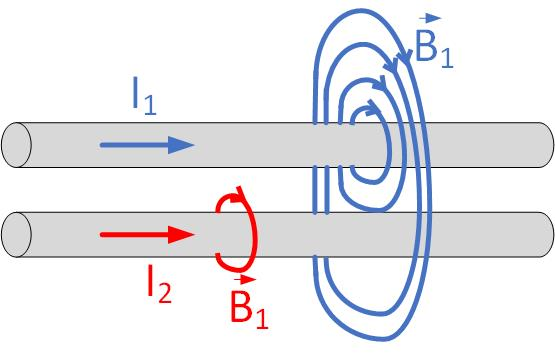
\includegraphics[scale=0.5]{../jpg/inductanceCurrentSameDir1.jpg}
\end{center}
\caption{Mutual Inductance: Increasing the magnetic field and therefore current in one wire due to another wire in vicinity. }
\label{MutualInduc2}
\end{figure}


In another example, in Figure \ref{MutualInduc1}, we have two currents, $I_1=1\,A$ and $I_2=1\,A$ flowing in the opposite directions. Current $I_1$ again produces four magnetic field lines, and current $I_2$ produces three magnetic field lines. Two of the magnetic field lines from conductor 1 encircle wire 2 as well. However, this time, the magnetic field lines flow in opposite directions. Therefore, the total number of magnetic field lines around conductor  2 is 3-2=1.  Therefore mutual inductance is $L_m=1/1=1\,H.$  When the magnetic field from two wires is in the opposite direction, fluxes subtract.


\begin{figure}[htbp]
\begin{center}
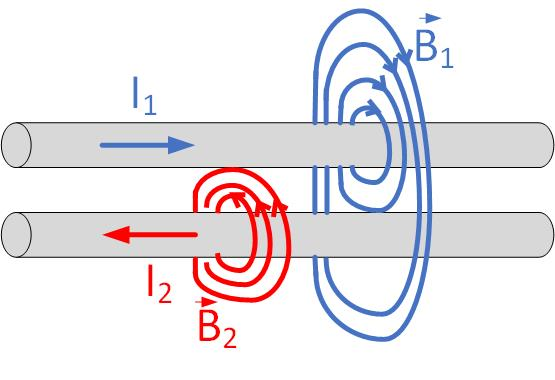
\includegraphics[scale=0.5]{../jpg/inductanceCurrentOppoDir1.jpg}
\end{center}
\caption{Mutual Inductance: Increasing the magnetic field and therefore current in one wire due to another wire in vicinity. }
\label{MutualInduc1}
\end{figure}

\end{document} 

